\subsection{Анализ исполнений}

В инструменте есть возможность анализа исполнений с помощью логирования. 

При нахождении нарушения инварианта происходит выход из перебора состояний, включение логирования и ещё одно исполнение последовательности доставок, нарушающих предикат. При этом выводится детализированный лог. Пример на рис.~\ref{fig:log} показывает фрагменты лога с нарушением линеаризуемости в однофазном ABD алгоритме (подчеркнуто красным).

Повторное исполнение последовательности доставок возможно благодаря детерминизму тестируемого кода.

\begin{figure}[h]
    \centering
    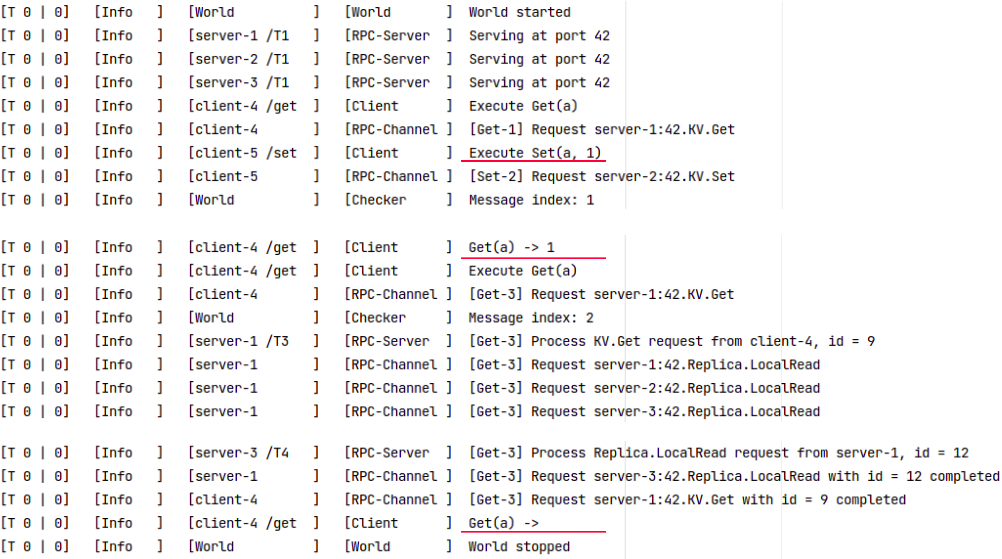
\includegraphics[width=\textwidth]{img/log.png}
    \caption{Лог для однофазного алгоритма с нарушением линеаризуемости}
    \label{fig:log}
\end{figure}
